\section{Dínamica general de las cotizaciones}
Comportamiento de los cotizantes (tdos los dependientes)
Comportamiento de algunas novedades  (variaciones anuales y mensuales) 2021, 2020 y 2019. Lo mismo retiros. Bajan los ingresos. Contraste con IEM */

cuerpo del documento mencionar variaciones anuales. Hablar de variaciones de solo un salario mínimo. 
 Variaciones mensuales con el total.
FABIO 
Tres hojas!  Capitulo 1 
1 - General con contraste ano tipo
2- Cotizantes por rango salarial
3 - Novedaes

\subsection{Índice Estacional Medio (IEM)}
Dejar el resultado general y el contraste con la estimación sin pandemia que usa el IEM, si toca incluir un parrafo general del IEM y de la estimación%

ANEXO- Dejar los insumos para el IEM (gráfico y tabla con multiplicadores)%

\begin{wrapfigure}{r}{12cm}
\label{fig:Cap22:Novedad_1}%
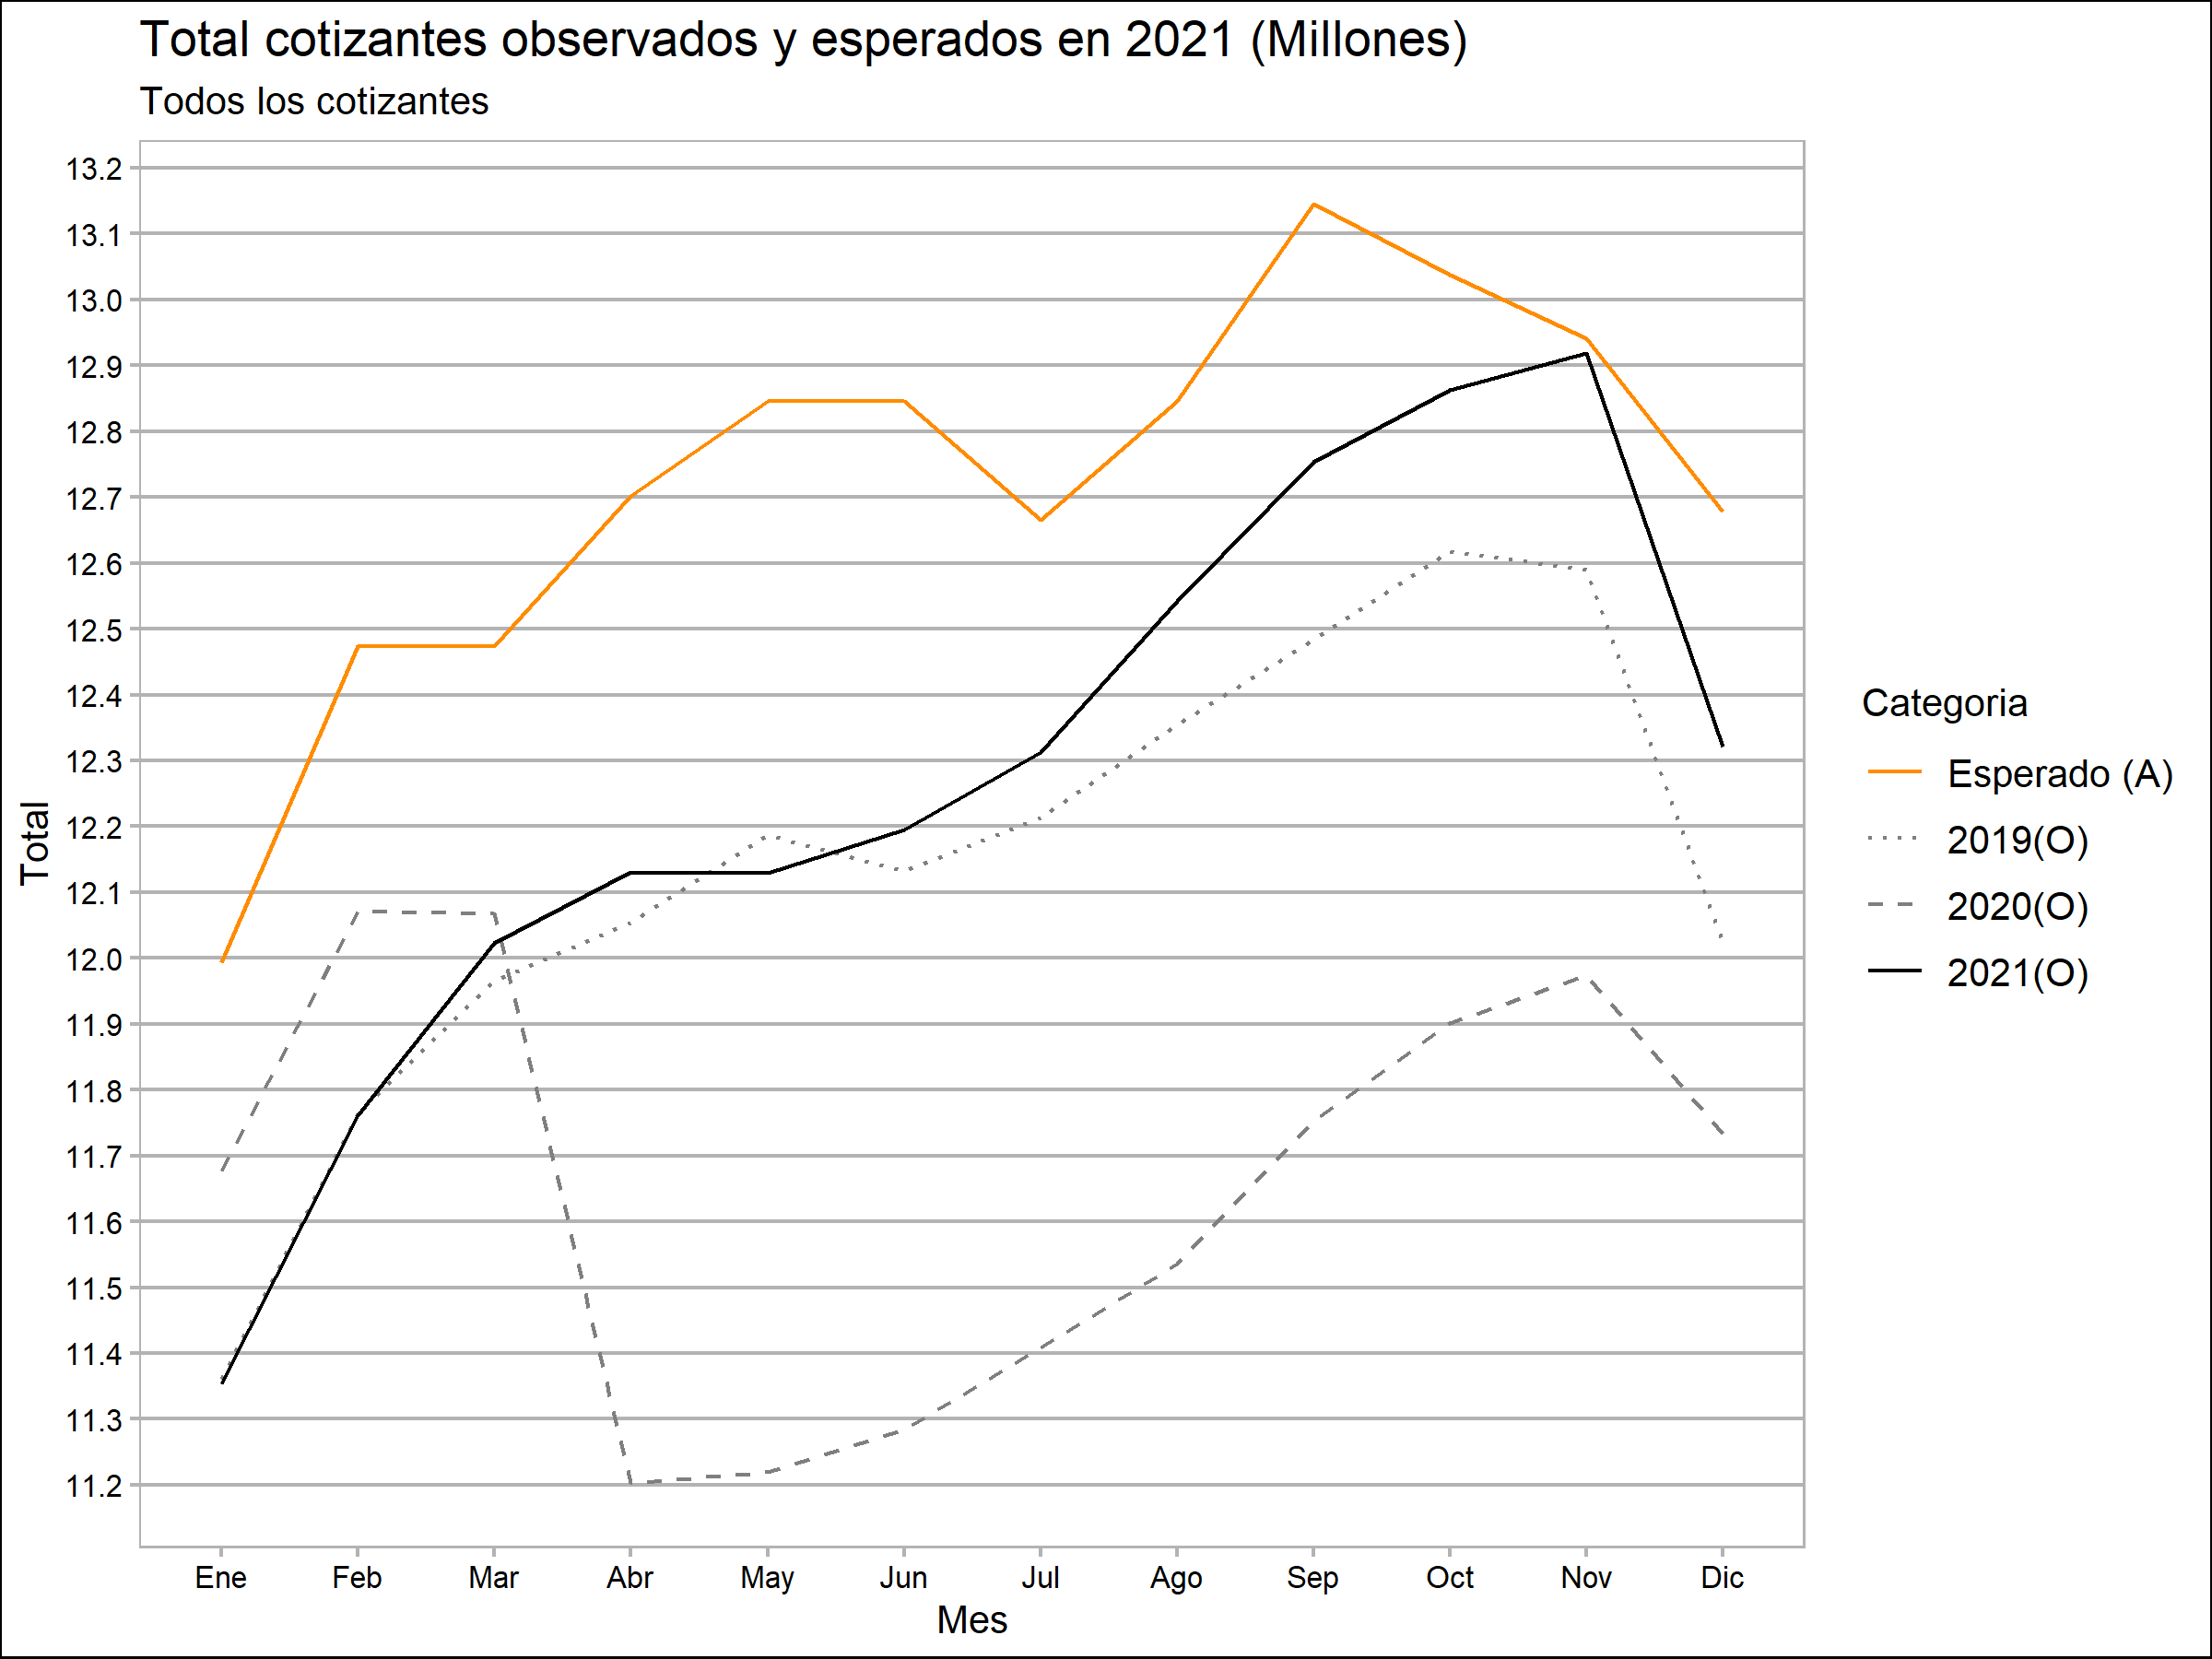
\includegraphics[width = 12.5cm]{figures/Capitulo_2_1/grafico_tot_1_1_1.png}
\caption{Total cotizantes observados y esperados en 2021}
\label{figura:IEM_Total}
\end{wrapfigure}
\lipsum[2-3]

\begin{intemize}
\item 
\end{intemize}

\begin{table}[!h]
\centering
\begin{minipage}{0.5\textwidth}
  \centering
  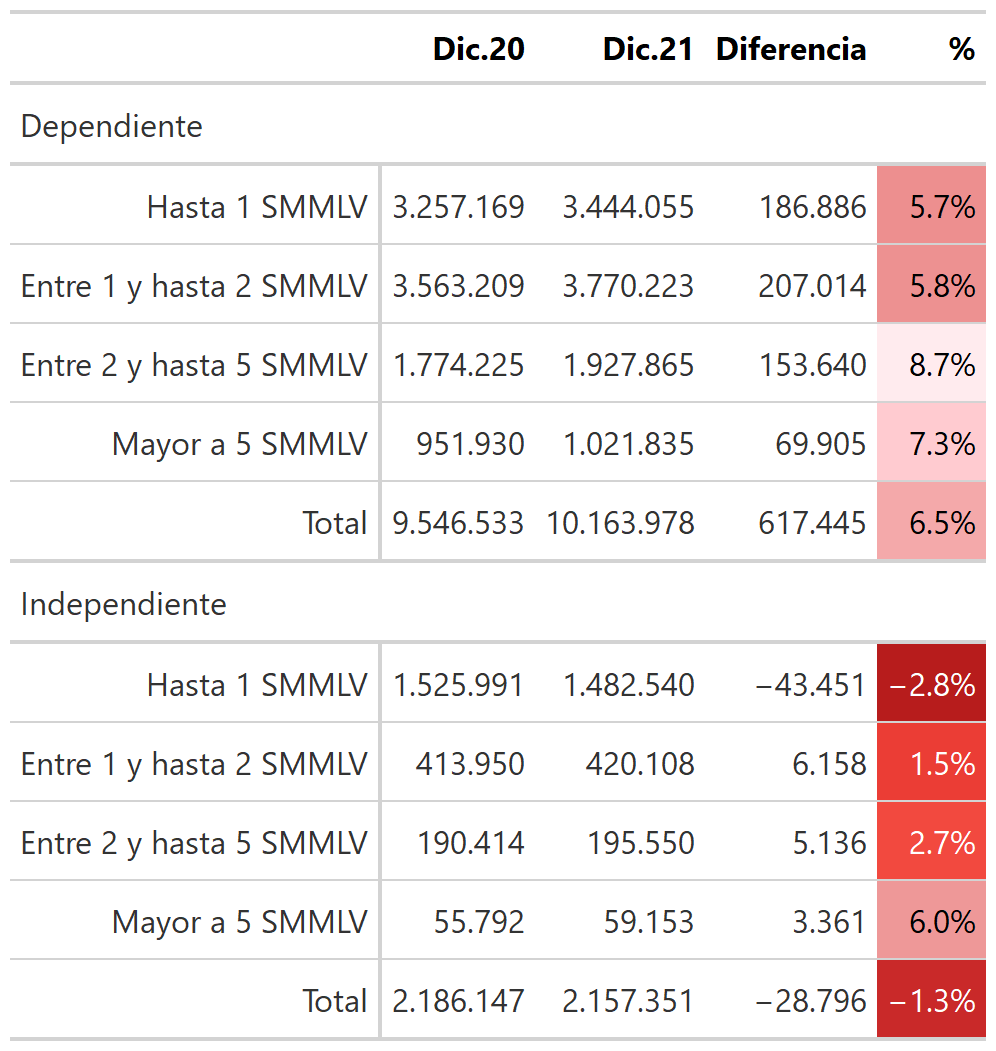
\includegraphics[width=0.6\linewidth]{results/Resumen/salida_table3_total.png}
\end{minipage}%
\begin{minipage}{0.5\textwidth}
  \centering
  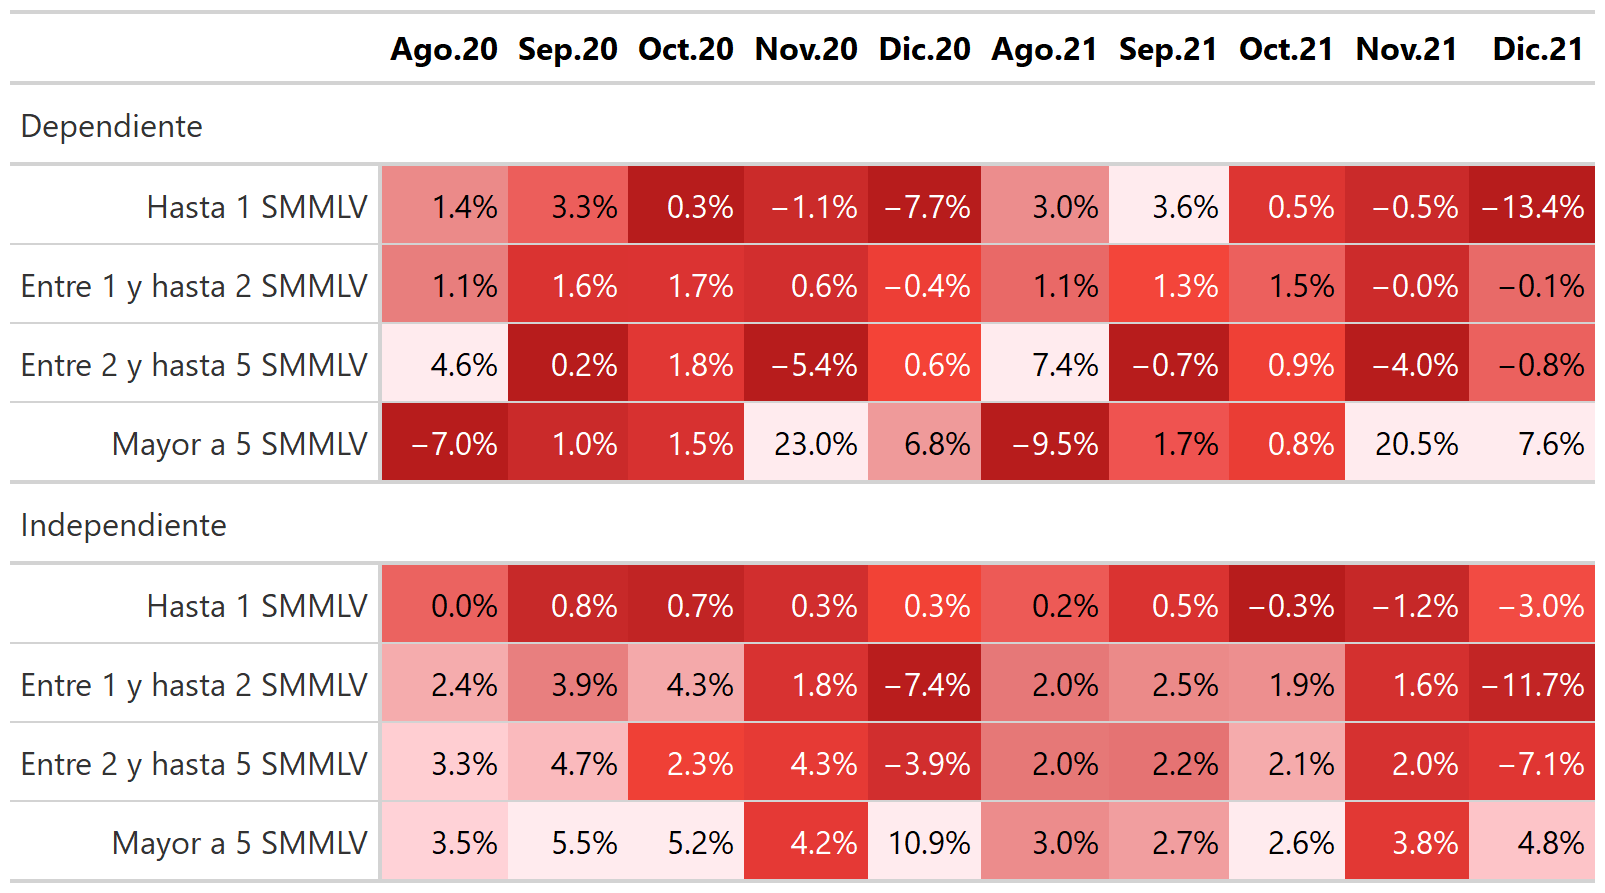
\includegraphics[width=\linewidth]{results/Resumen/salida_table3_variaciones.png}
\end{minipage}
\caption{Resumen número de cotizantes por rango salarial (IBC)}. Totales (Izq.), variaciones mensuales (Der.)
\label{tabla:tabla3}
\end{table}


\subsection{Novedades}


\begin{wrapfigure}{r}{0.6\textwidth}
\label{fig:Cap22:Novedad_1}%
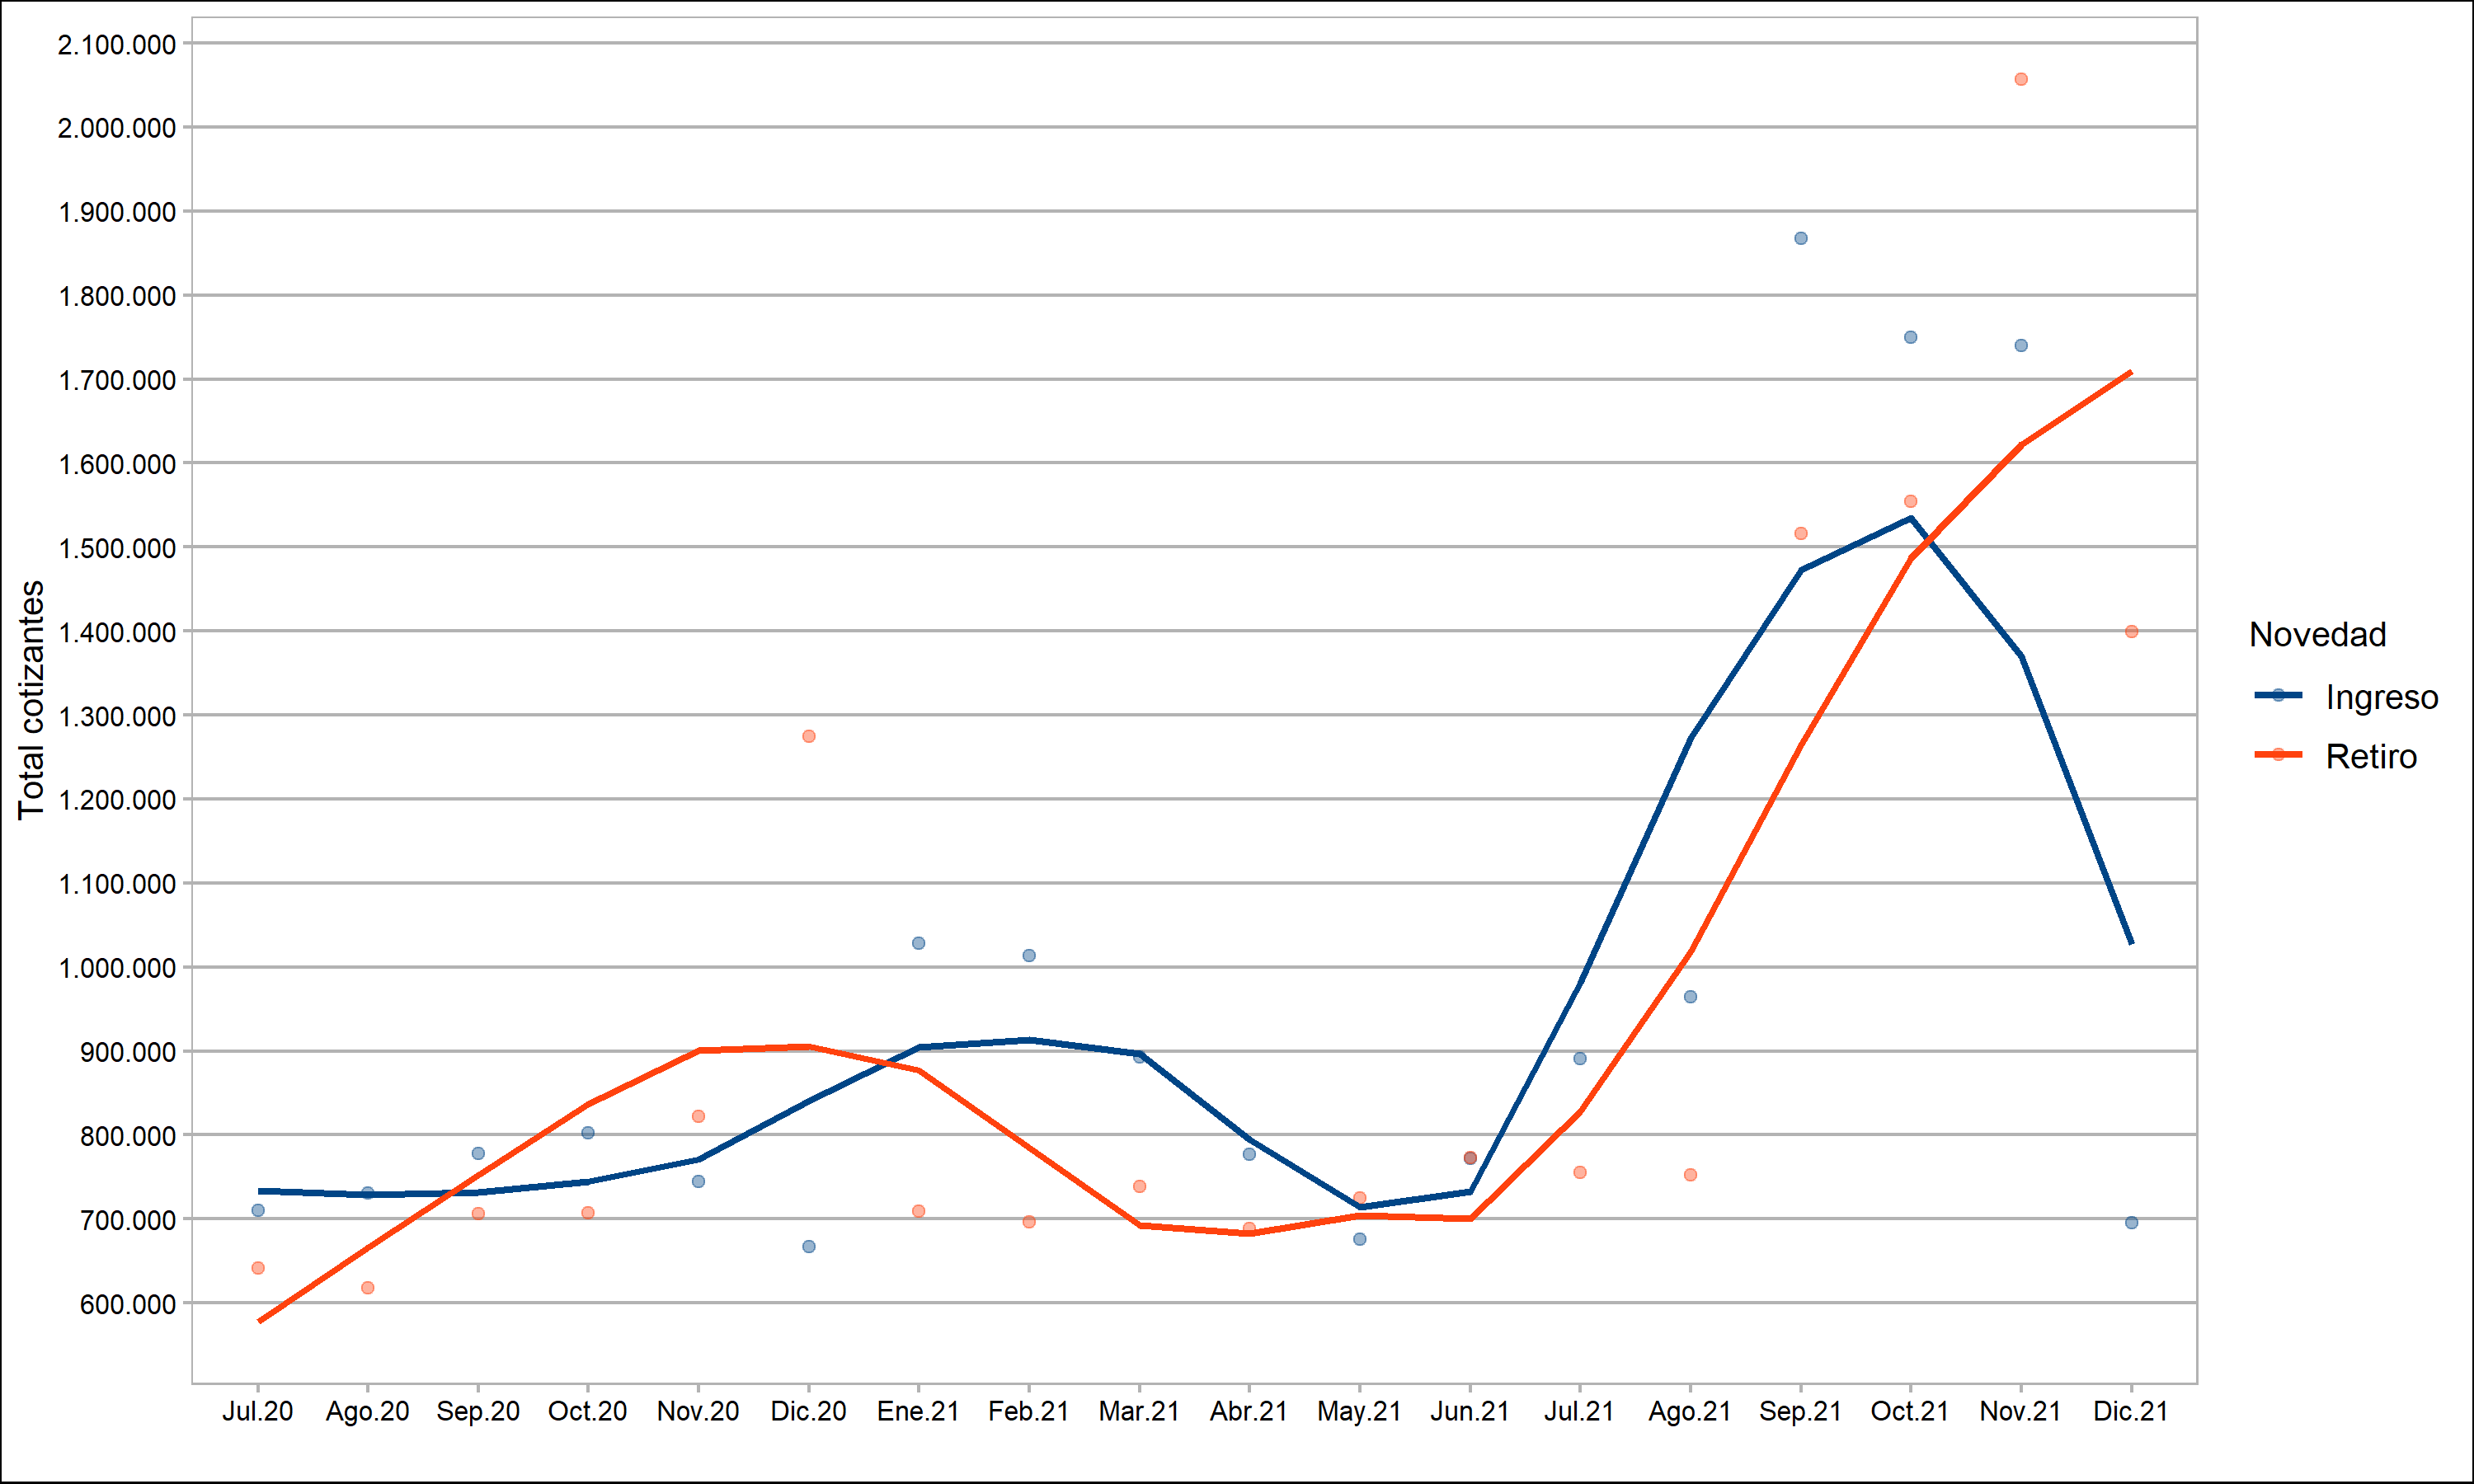
\includegraphics[width = 11.5cm]{figures/Capitulo_2_2/total_novedades_dependientes_1.png}
\caption{Comparación del total de novedades para dependientes (ingresos, retiros)}
\label{figura:novedad:sectorprivado:IR}
\end{wrapfigure}

\lipsum[2-4]

\begin{wrapfigure}{l}{0.6\textwidth}
\label{fig:Cap22:Novedad_2}
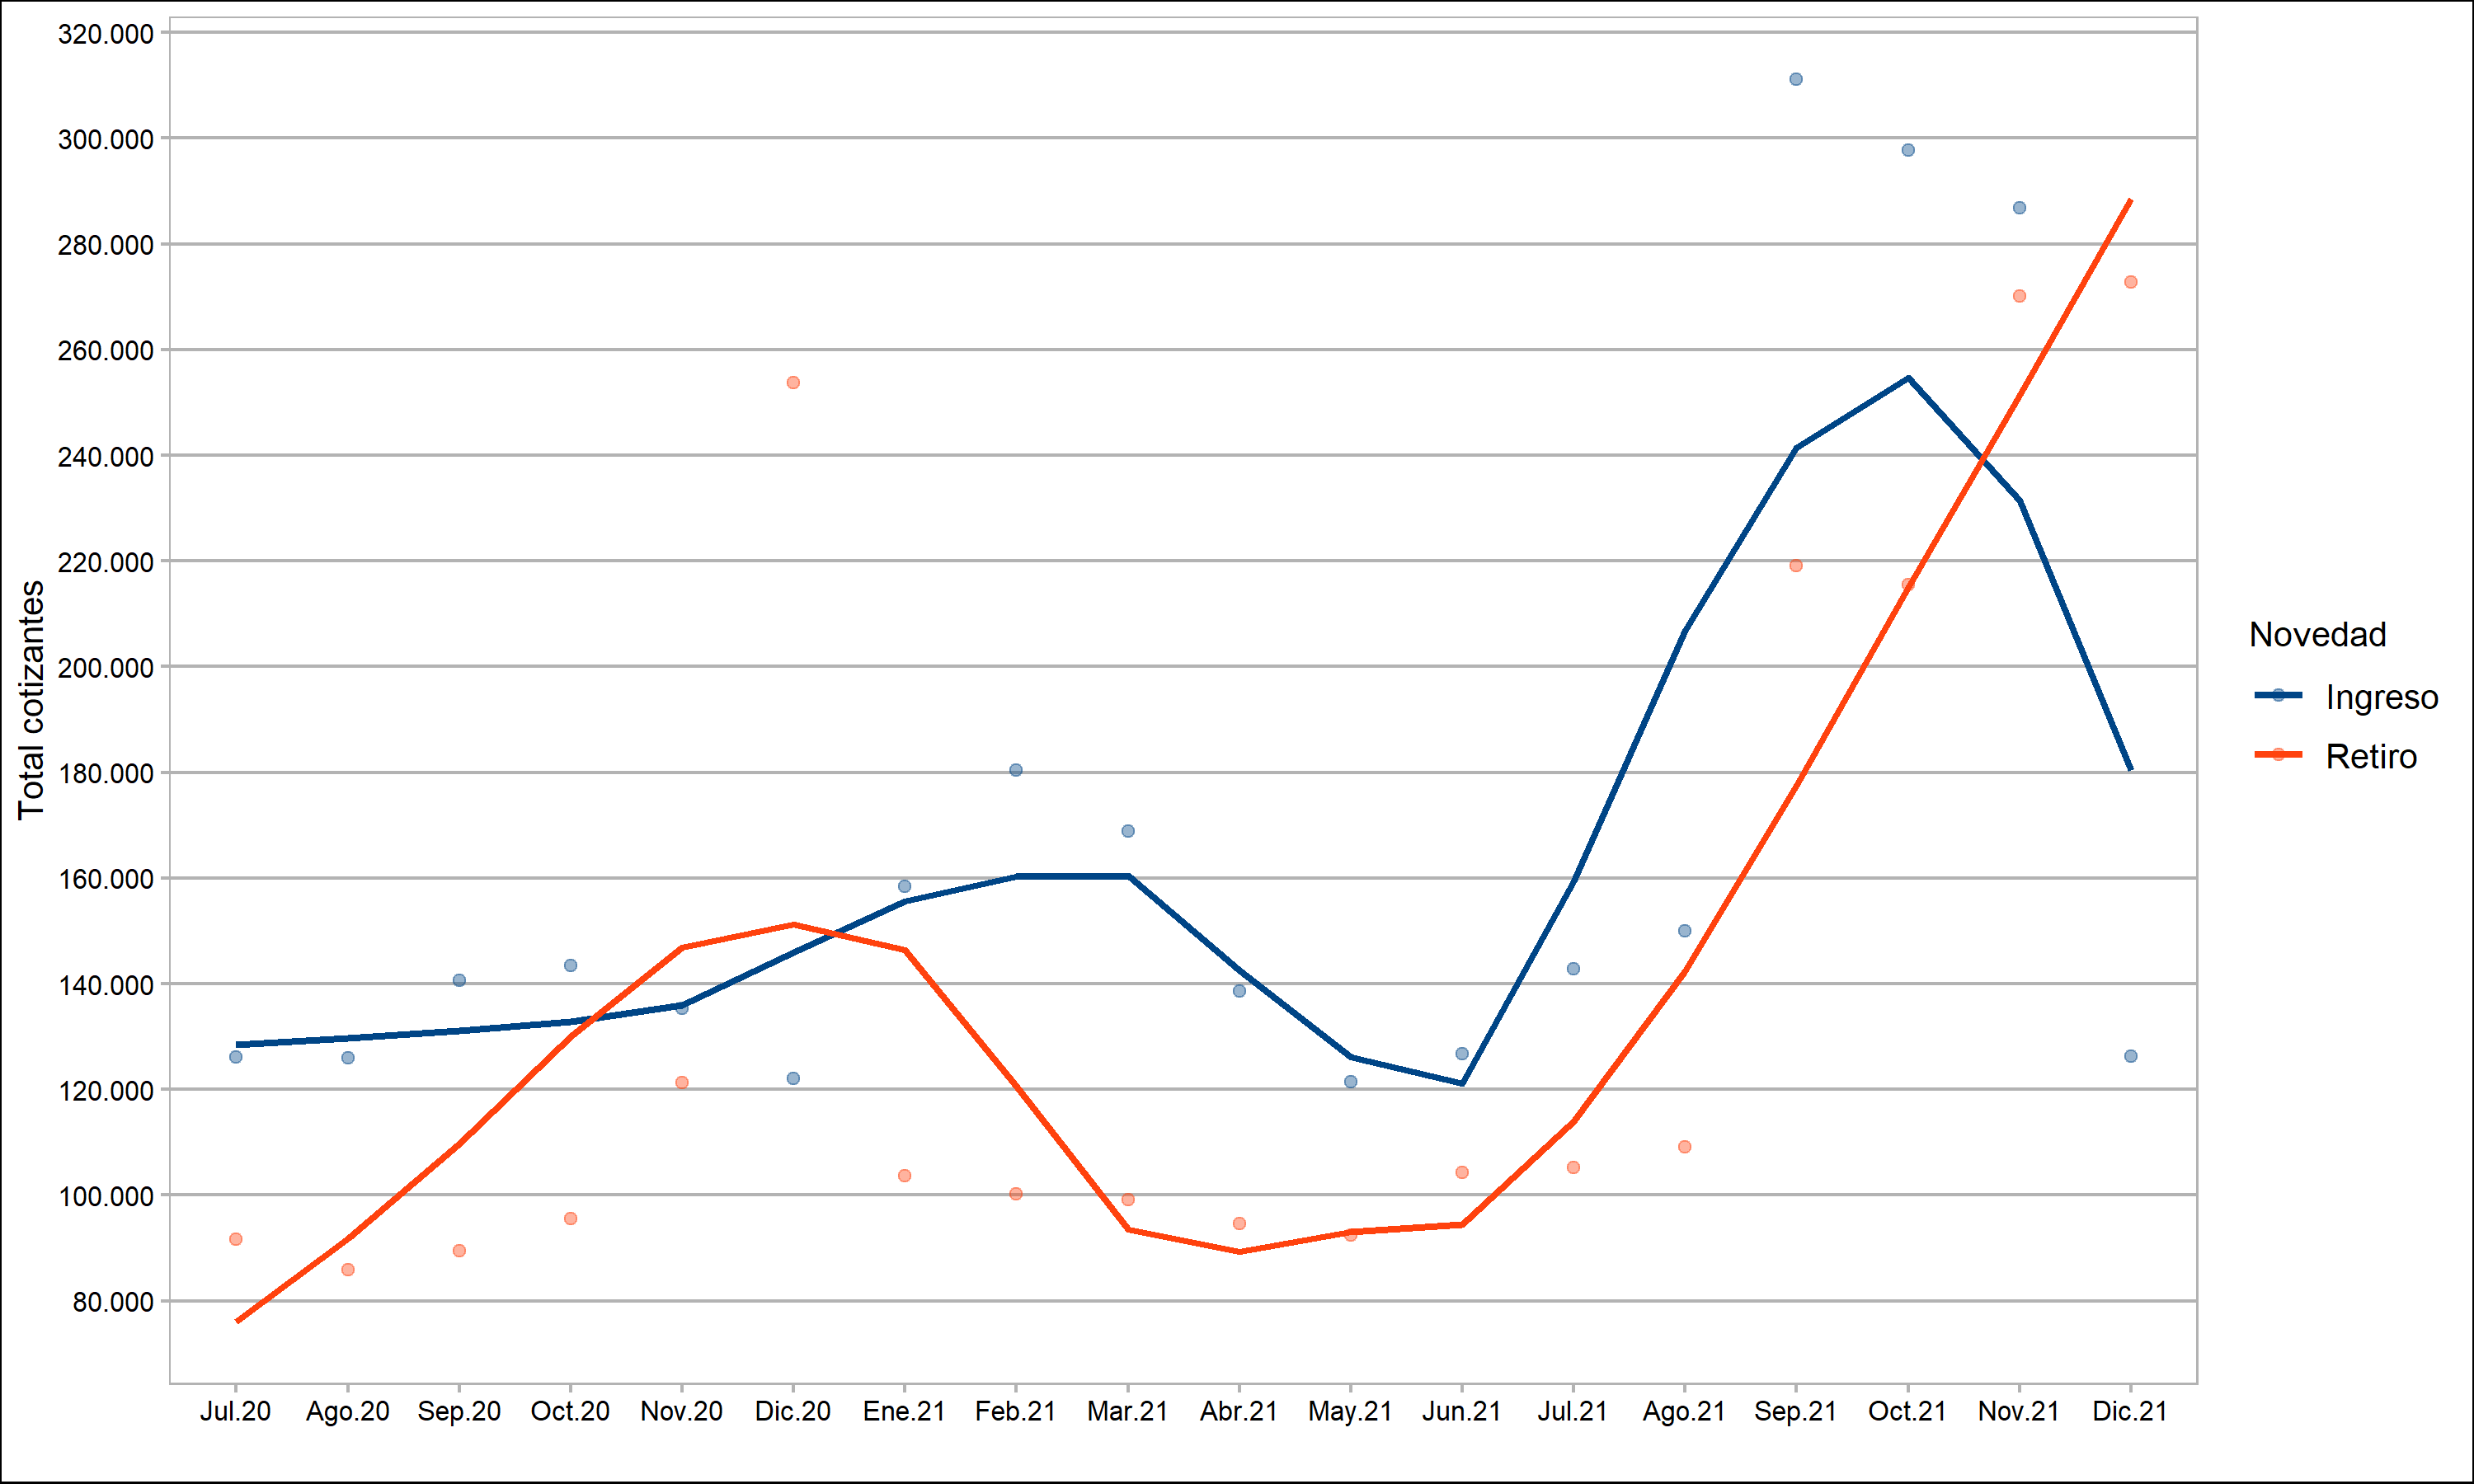
\includegraphics[width = 11.5cm]{figures/Capitulo_2_2/total_novedades_independientes_1.png}
\caption{Comparación del total de novedades para independientes}
\label{figura:novedad:sectorprivado:IR}
\end{wrapfigure}

\lipsum[2-5]

\begin{table}[!h]
\centering
\begin{minipage}{0.5\textwidth}
  \centering
  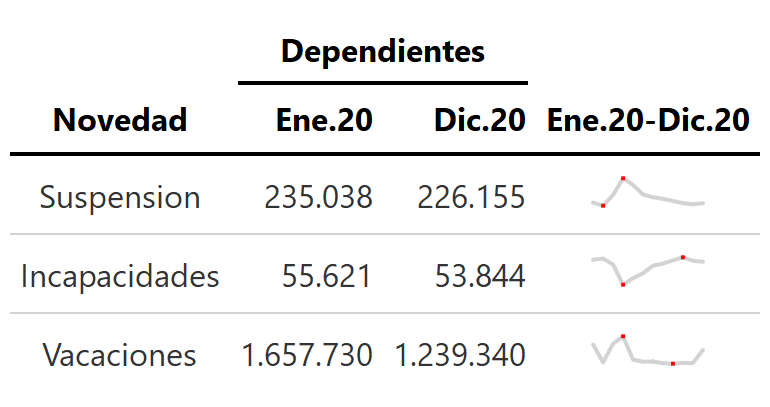
\includegraphics[width=\linewidth]{results/Cotizantes_Novedades/salida_dependientes_novedades_resto_comparativo.png}
\end{minipage}%
\begin{minipage}{0.5\textwidth}
  \centering
  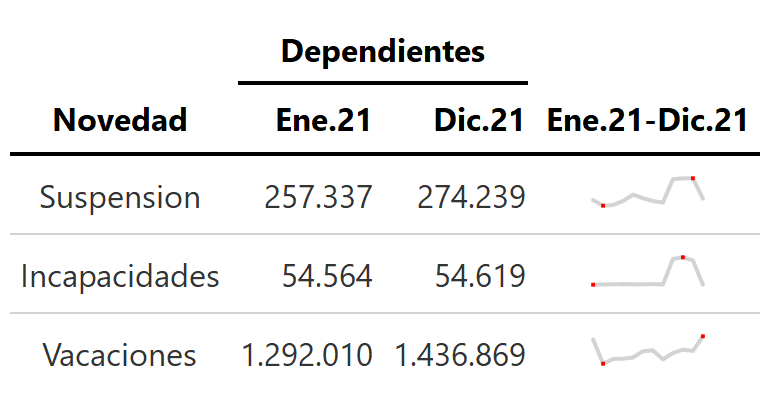
\includegraphics[width=\linewidth]{results/Cotizantes_Novedades/salida_dependientes_novedades_resto.png}
\end{minipage}
\caption{Total novedades y tendencia anual}
\label{tabla:tabla3}
\end{table}
\lipsum[2-3] %%%
